\documentclass{beamer}

\usepackage{fontspec} 
% \usepackage{lsp-makros}
\useoutertheme{lsp}

\usepackage{lsptitle}

\def\two@digits#1{\ifnum#1<10 0\fi\number#1}
\def\mytoday{\two@digits{\number\day}.\two@digits{\number\month}.\number\year}


\usepackage{xspace,multicol}
\newcommand{\latex}{\LaTeX\xspace}
\usepackage{tikz}


\newcounter{lastpagemainpart}
\footnotesep0pt
\renewcommand{\footnoterule}{}
\usefootnotetemplate{
  \noindent
  \insertfootnotemark\insertfootnotetext}

\let\beamerfn=\footnote
\renewcommand{\footnote}[1]{%
\let\oldfnsize=\footnotesize%
\let\footnotesize=\tiny%
\beamerfn<\thebeamerpauses->{#1}%
\let\footnotesize=\oldfnsize}


\date{Open Access and share your knowledge\\2022-11-02}

\usepackage{eurosym}  
 
\renewcommand{\centerline}[1]{\hfill#1\hfill\hfill\mbox{}}


\title{Open access books\newline in African linguistics}
% \institute{FU Berlin}
\author[LangSci]{Sebastian Nordhoff}



\begin{document}
\lspbeamertitle

\section{Introduction}
\frame{
\frametitle{Introduction:\strut\\ Sebastian Nordhoff}
%   \includegraphics[height=.2\textheight]{./path/to/graphicsfile}
  \begin{itemize}
    \item  lives in Western Europe
    \item  worked on languages of South America (Guarani) and Asia (Sri Lanka Malay)
    \item 4 books, 30+ scholarly articles
    \item since 2014 managing director of Language Science Press
  \end{itemize}
}

\frame{
\frametitle{Introduction:\strut\\ Language Science Press}
%   \includegraphics[height=.2\textheight]{./path/to/graphicsfile}
  \begin{itemize}
    \item scholar-led Open Access publisher
    \begin{itemize}
      \item CC-BY licenses
    \end{itemize}
    \item \textbf{no fees for readers}
    \item \textbf{no fees for authors}
    \item funded by a network of 100+ institutions worldwide
    \begin{itemize}
      \item \url{https://langsci-press.org/sponsors}
      \item running costs of about 120k€/year (≃4k€/book)
    \end{itemize}
    \item 30 series ranging from laboratory phonology to translation studies
    \item 200+ books up to date
    \begin{itemize}
      \item 30 books/year
      \item 100--1600 pages
    \end{itemize}

    \item 1000+ authors
  \end{itemize}
}

\frame{
\frametitle{Introduction:\strut\\ Language Science Press}
  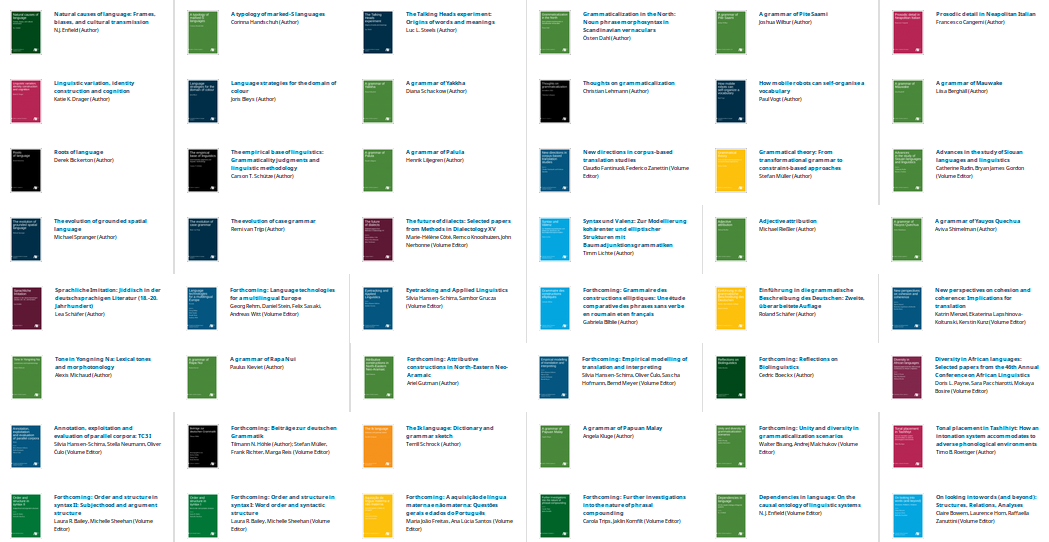
\includegraphics[height=\textheight]{catalog.png}
}

\section{Books}
\frame{
\frametitle{Availability}
%   \includegraphics[height=.2\textheight]{./path/to/graphicsfile}
  \begin{itemize}
    \item  pdfs from \url{langsci-press.org} for free
    \item  paper books in book stores and Amazon for about 30-60 EUR
    \item GoogleBooks, DOAB, OAPEN, VLB, PaperHive
    \item Zenodo, AfricArXiv
  \end{itemize}
}

% \frame{
% \frametitle{Roads to Open Access}
% %   \includegraphics[height=.2\textheight]{./path/to/graphicsfile}
%   \begin{itemize}
%     \item  \textbf{The Green Road}: repositories
%     \item \textbf{The Golden Road}: author pays
%     \item \textbf{The Diamond Road}: community pays
%   \end{itemize}
% }

% \section{Articles}
% \frame{
% \frametitle{The Green Road}
% %   \includegraphics[height=.2\textheight]{./path/to/graphicsfile}
%   \begin{itemize}
%     \item Choose a traditional journal
%     \item Get your article accepted
%     \item The journal publishes and monetizes your article as usual
%     \item You deposit a version of the article in a depository of your university or a repository of your discipline
%     \begin{itemize}
%       \item publisher regulation vary as to which version (submitted, accepted, published) you can deposit
%       \item check Sherpa Romeo https://v2.sherpa.ac.uk/romeo/search.html
%     \end{itemize}
%   \end{itemize}
% }
%
% \frame{
% \frametitle{Sherpa Romeo}
%   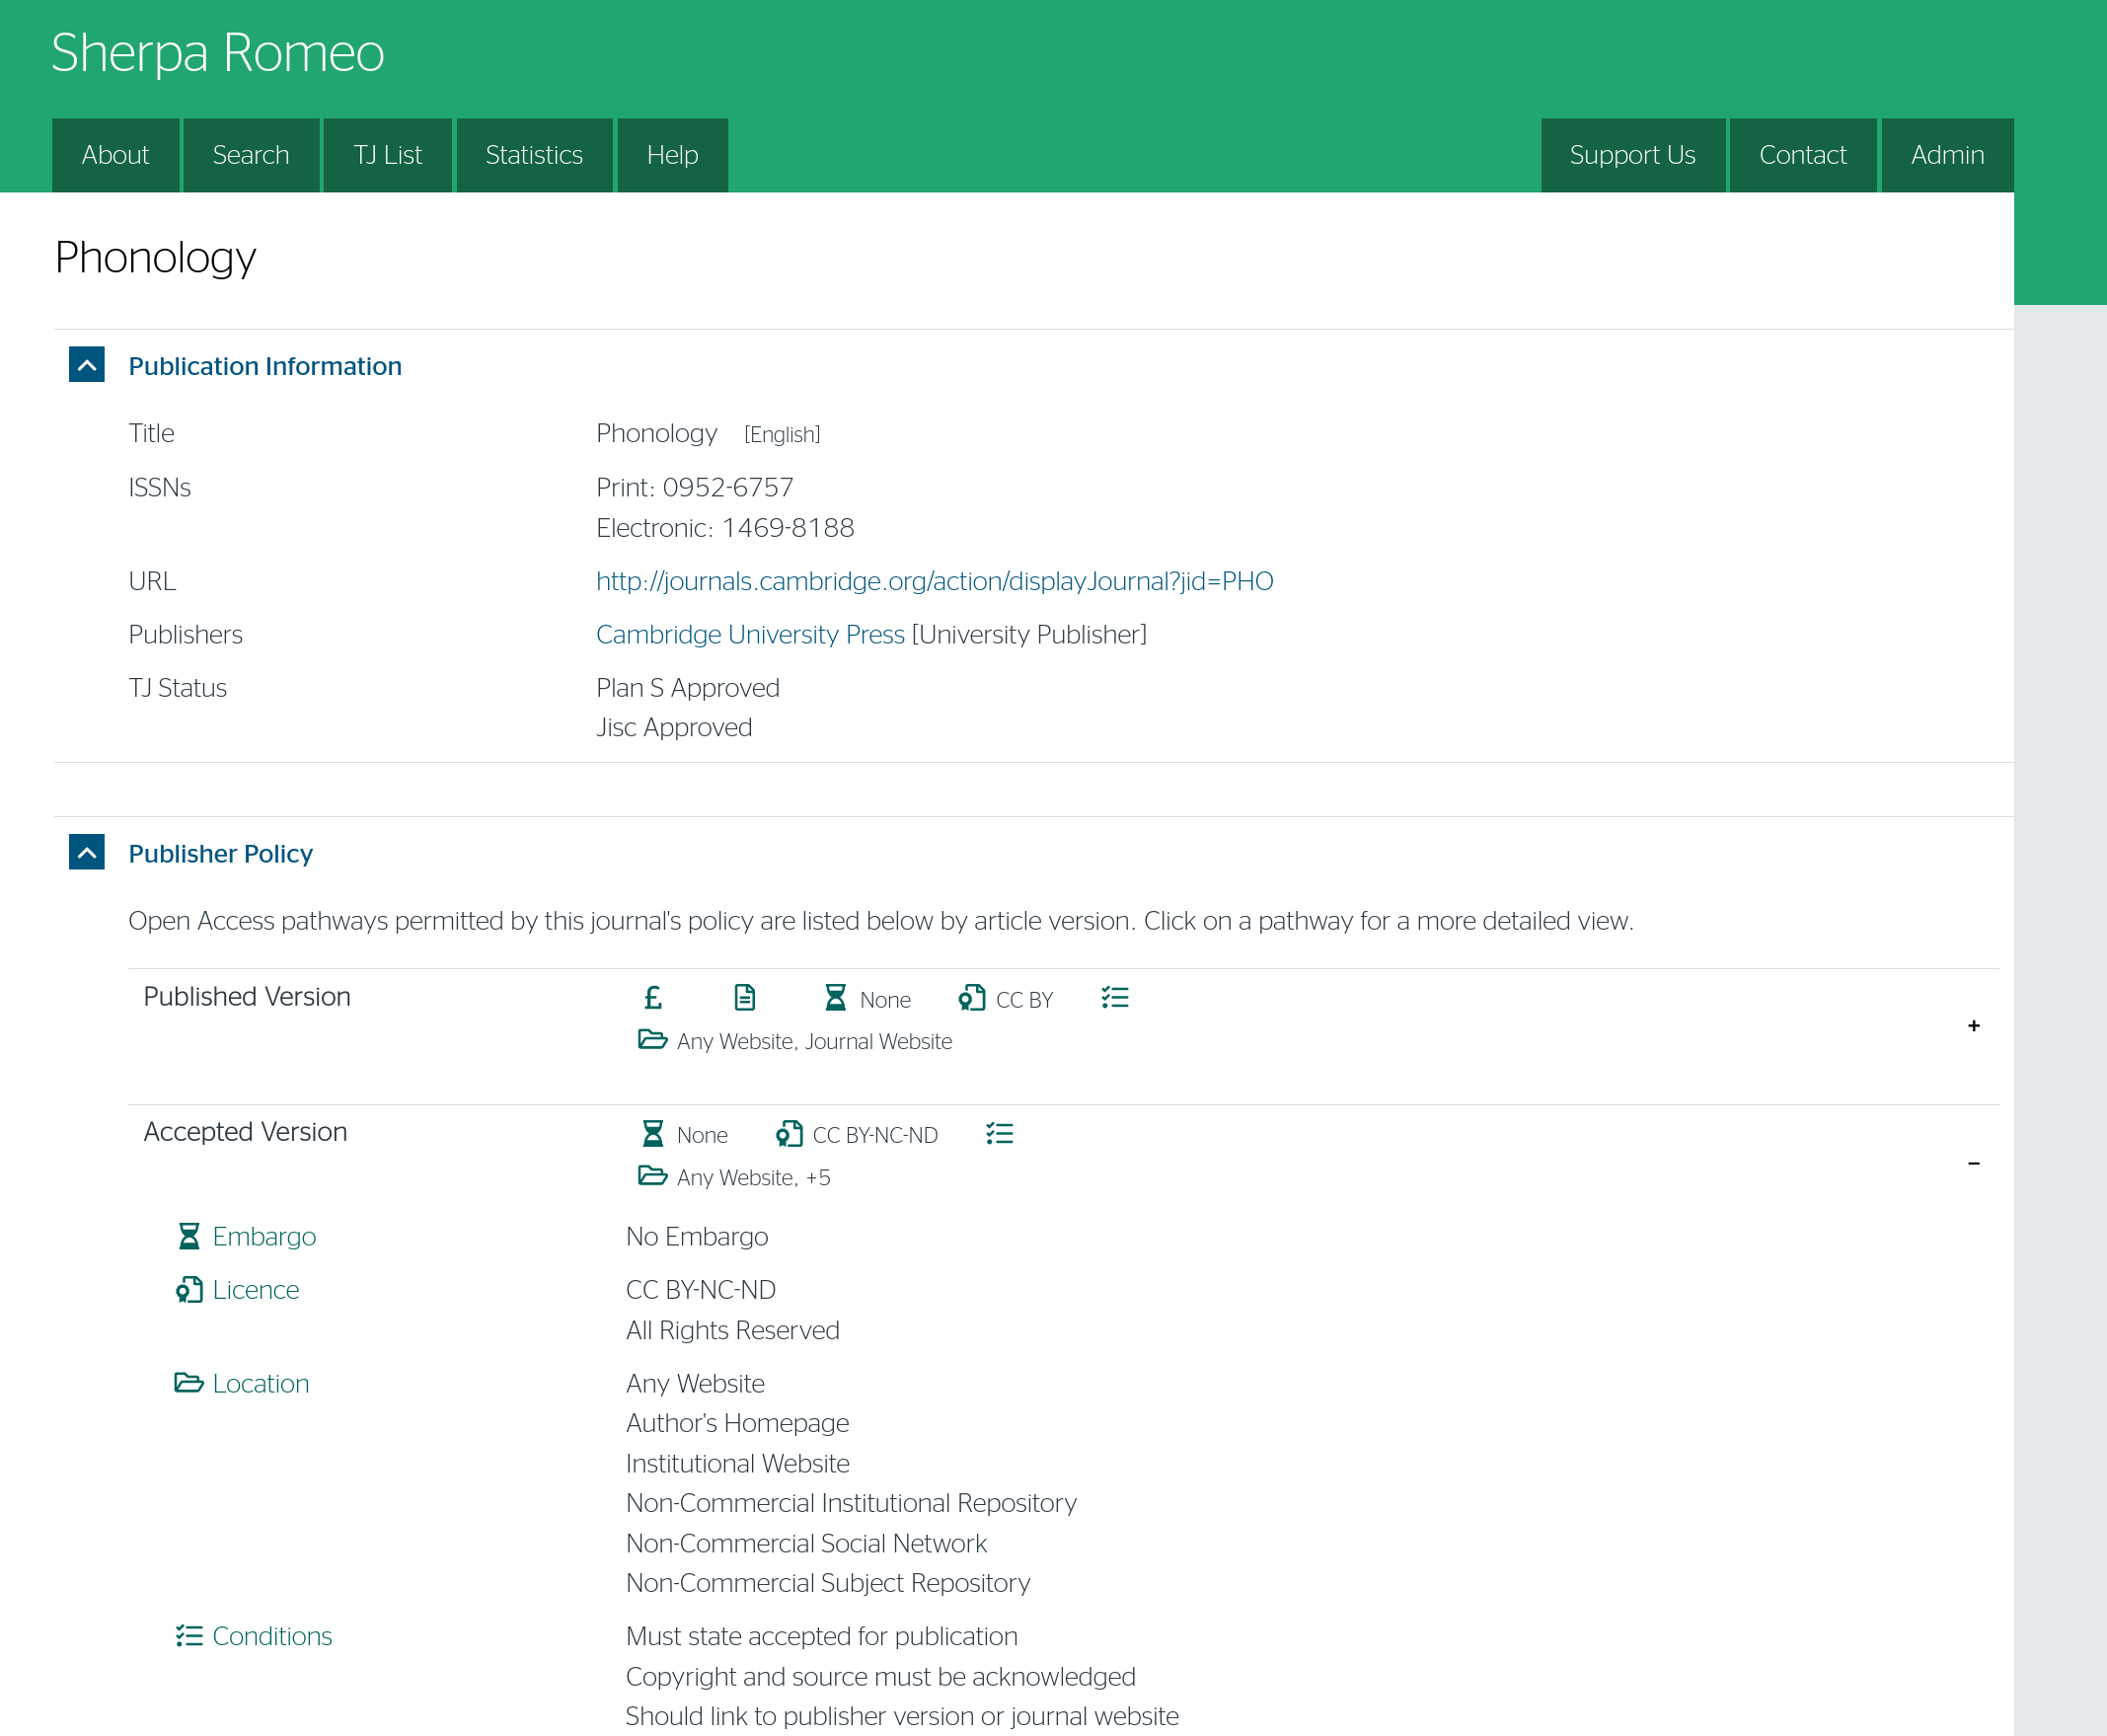
\includegraphics[height=1\textheight]{sherparomeo.png}
% }
%
% \frame{
% \frametitle{The Golden Road}
% %   \includegraphics[height=.2\textheight]{./path/to/graphicsfile}
%   \begin{itemize}
%     \item Select a journal
%     \item Get your paper accepted
%     \item Pay a fee
%     \begin{itemize}
%       \item article: 300 USD -- 3.000 USD
%       \item book: 5.000 -- 25.000 USD
%     \end{itemize}
%     \item Readers don't have to pay anything to read the article
%     \item Beware of predatory journals!
%     \item Check the Directory of Open Access Journals (DOAJ)
%     \item thinkchecksubmit.org
%   \end{itemize}
% }
%
% \frame{
% \frametitle{Predatory Journals}
%   
\includegraphics[height=.45\textheight]{predatoryjournal.png}
% }
%
%
% \frame{
% \frametitle{DOAJ}
%   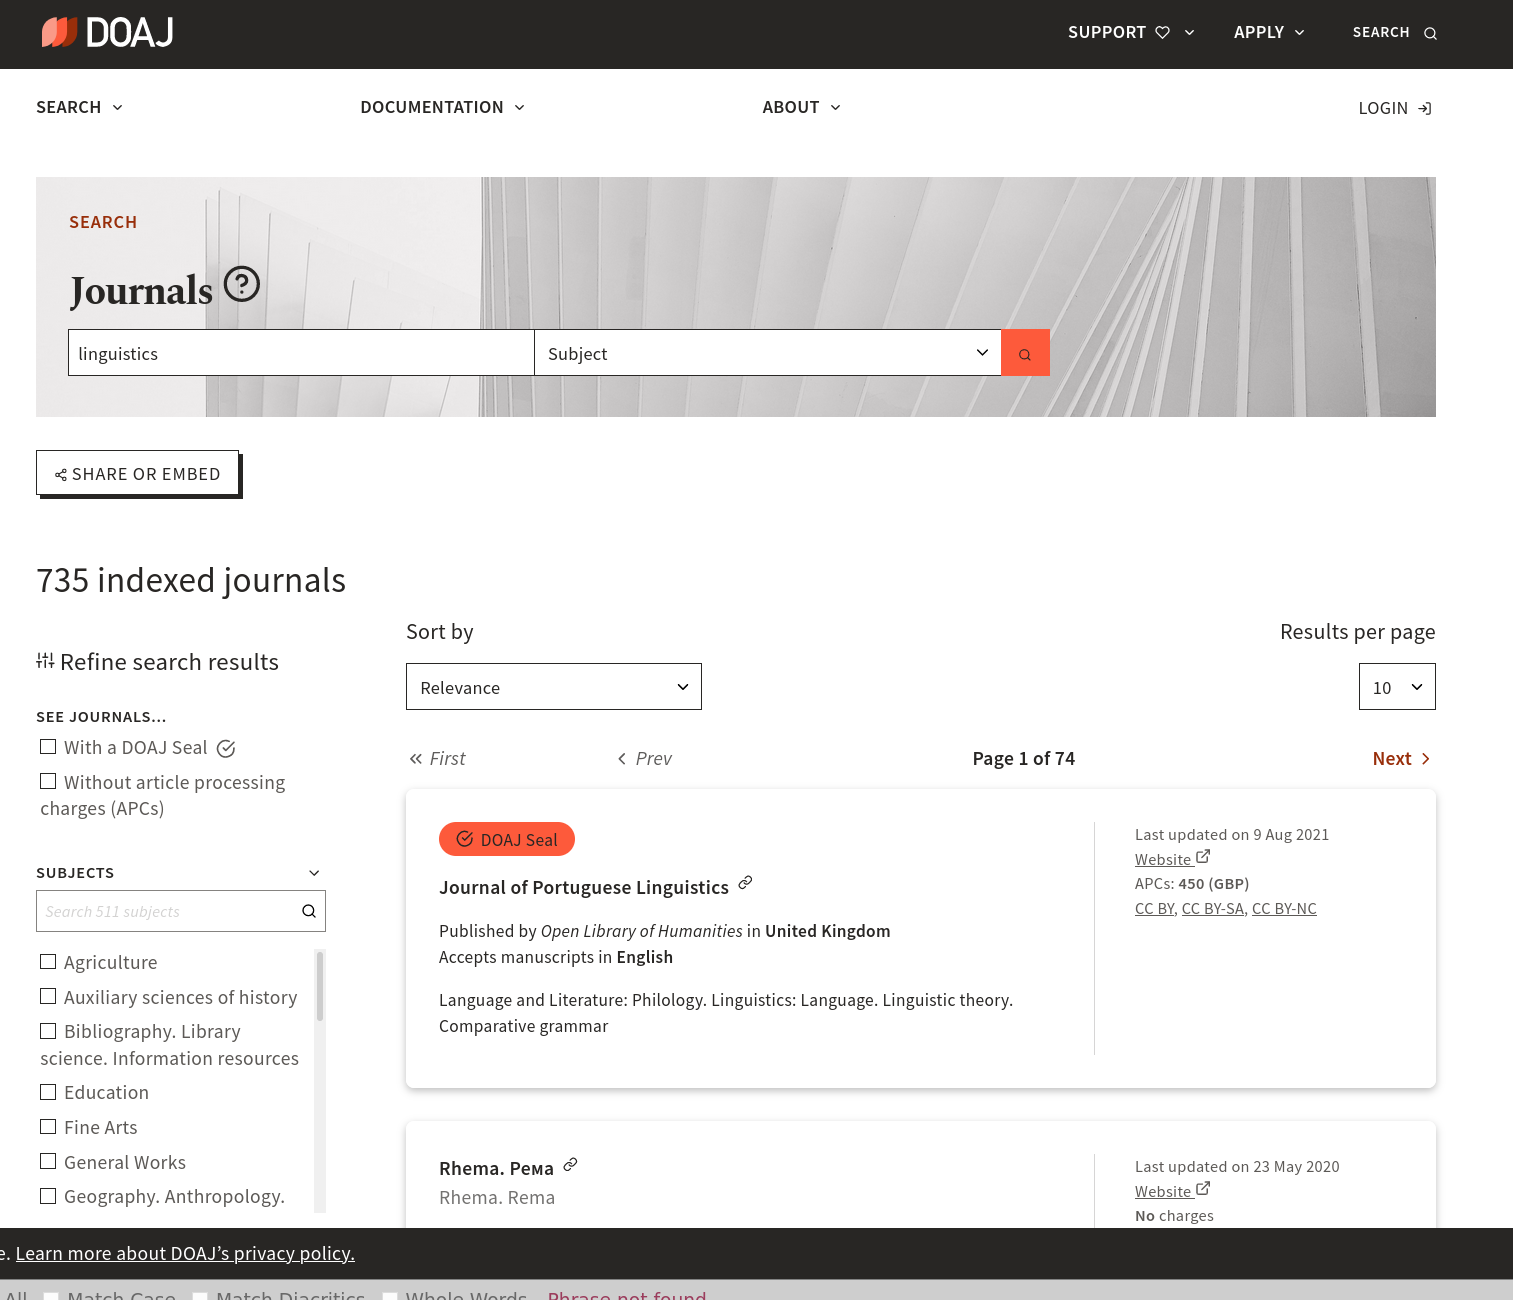
\includegraphics[height=1.2\textheight]{doaj.png}
% }
%
% \frame{
% \frametitle{The Diamond Road\strut\\(also called Platinum)}
% %   \includegraphics[height=.2\textheight]{./path/to/graphicsfile}
%   \begin{itemize}
%     \item Select a journal
%     \item Get your paper accepted
%     \item Pay \textbf{no} fee
%     \item Readers don't have to pay anything to read the article
%     \item A list of Diamond OA journals for linguistics can be found on oaling.wordpress.com
%   \end{itemize}
% }
%
%
% % \frame{
% % \frametitle{Think Check Submit}
% %   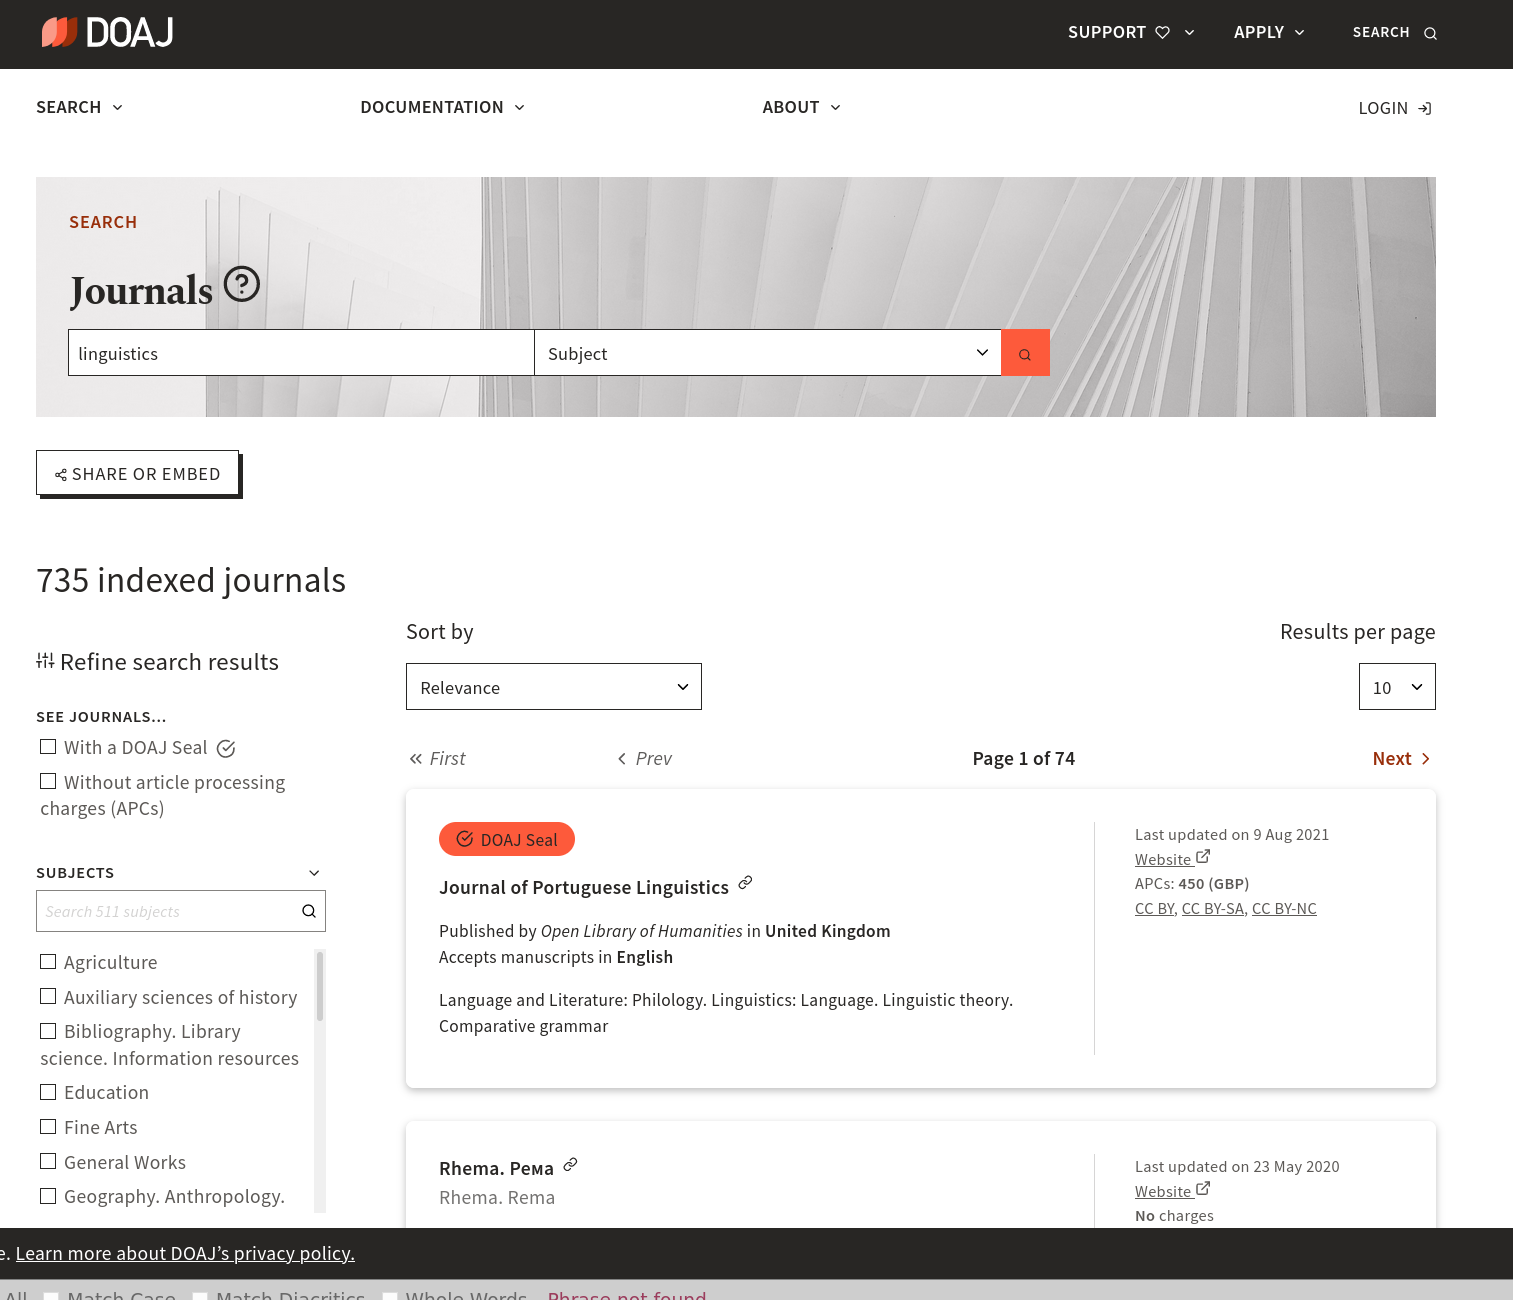
\includegraphics[height=\textheight]{doaj.png}
% % }
%
% \section{Books}
\frame{
\frametitle{Open Access books at\\ Language Science Press}
%   \includegraphics[height=.2\textheight]{./path/to/graphicsfile}
\begin{columns}
\column{7cm}
\begin{itemize}
    \item African Language Grammars and Dictionaries
    \begin{itemize}
      \item Dictionary + sketch grammar
      \item Grammar + word list.
      \item https://langsci-press.org/catalog/series/algad
    \end{itemize}
    \item Niger-Congo Comparative Studies
    \begin{itemize}
      \item https://langsci-press.org/catalog/series/nccs
    \end{itemize}
    \item Contemporary African Linguistics (from the Association for Contemporary African Linguistics)
    \begin{itemize}
      \item https://langsci-press.org/catalog/series/cal
    \end{itemize}
  \end{itemize}
\column{3cm}
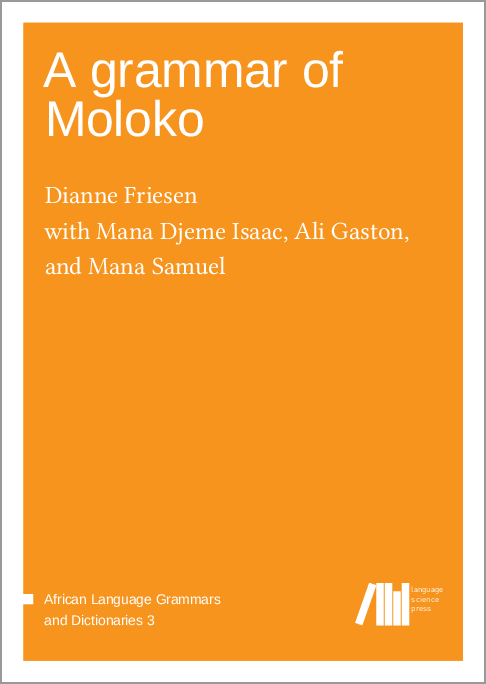
\includegraphics[height=2.2cm]{algad.png}\\
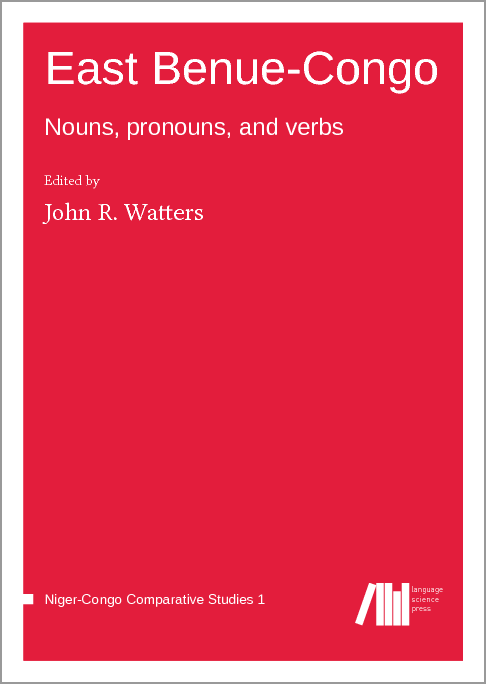
\includegraphics[height=2.2cm]{mcnc.png}\\
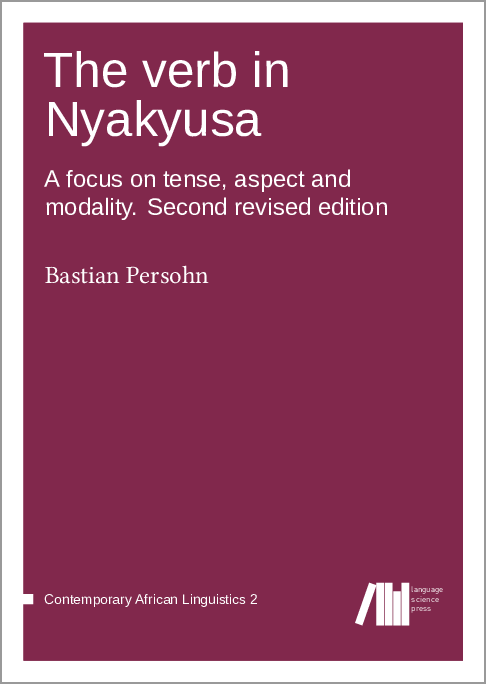
\includegraphics[height=2.2cm]{cal.png}
\end{columns}
}


\frame{
\frametitle{Quantity:\newline downloads}
  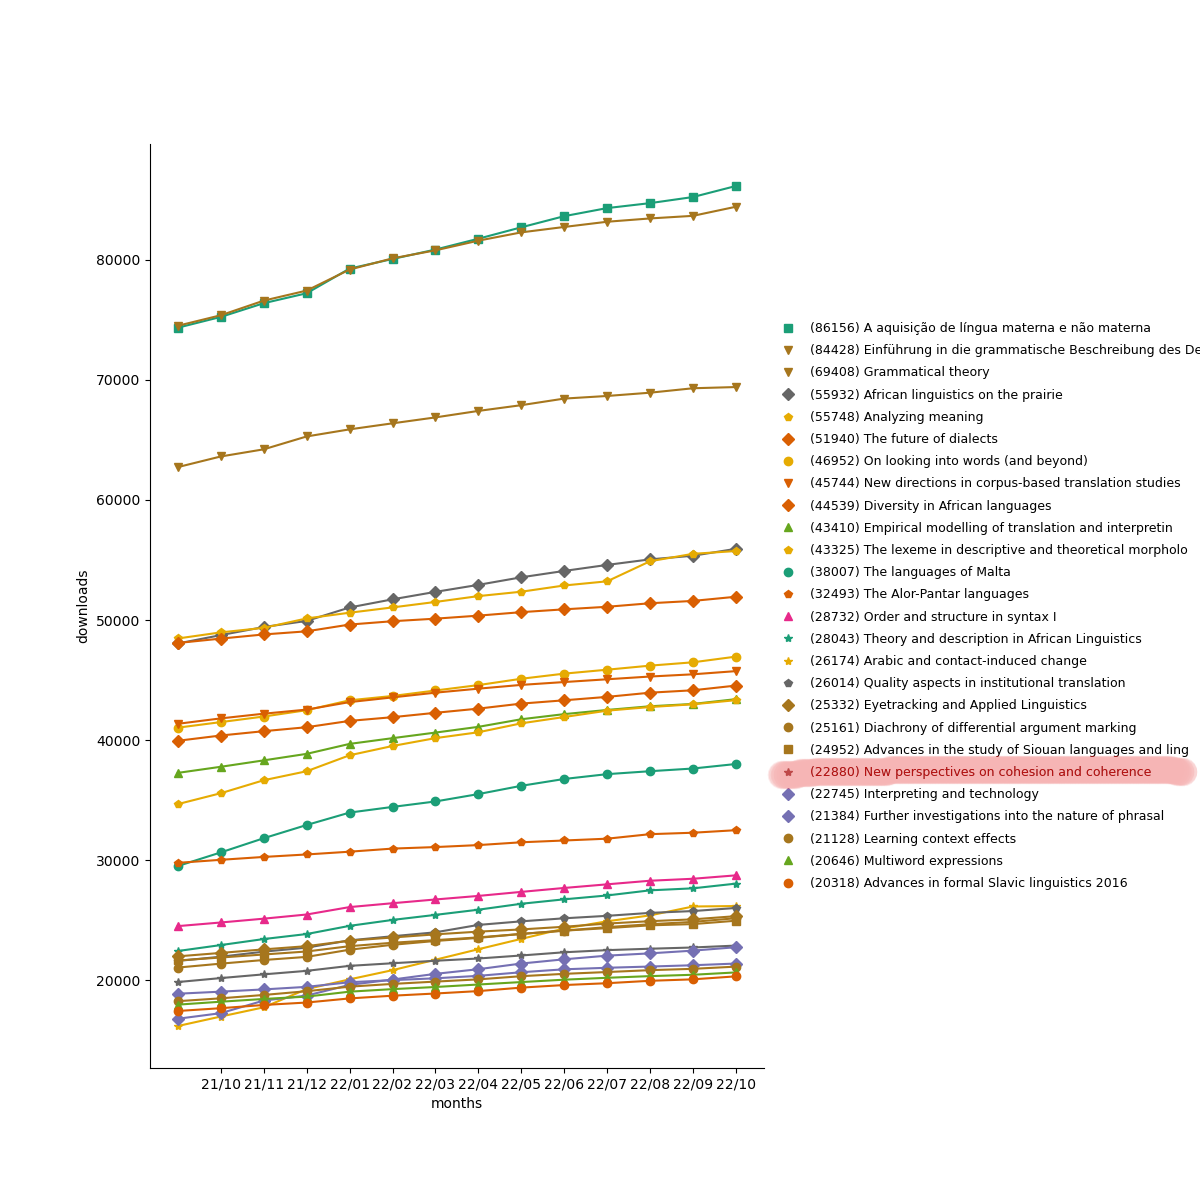
\includegraphics[height=1.5\textheight]{cumulativeallultrahigh.png}
}

\frame{
\frametitle{Quality:\newline\mbox{Leonard Bloomfield Award 2023}}
%   \includegraphics[height=.2\textheight]{./path/to/graphicsfile}
\begin{columns}
 \column{5cm}
  \begin{itemize}
    \item  Awarded by the \textit{Linguistic Society of America} for the best book of the year
    \item This book is about an African language, but appeared in a non-areal series (\textit{Comprehensive Grammar Library})
  \end{itemize}
  \column{4cm}
  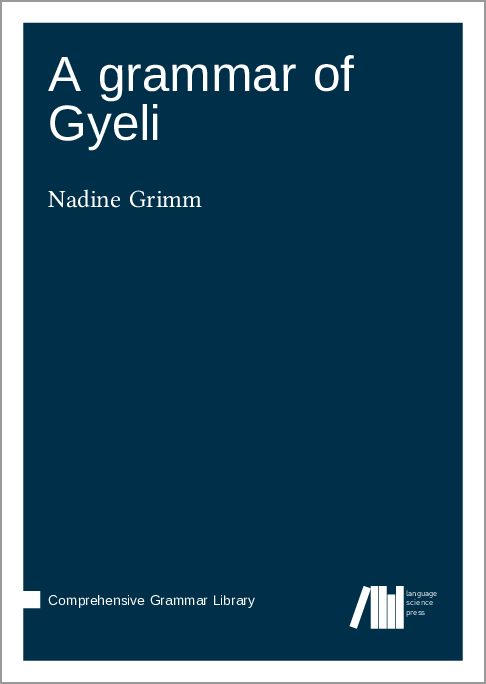
\includegraphics[height=.8\textheight]{gyelibook.png}
\end{columns}
}

\section{Interaction}
\frame{
\frametitle{How to submit a book\strut\\ proposal}
%   \includegraphics[height=.2\textheight]{./path/to/graphicsfile}
  \begin{itemize}
    \item  identify relevant series and check their websites
    \begin{itemize}
      \item aims and scope
      \item requirements
      \item processes for proposals might be specified (or not)
    \end{itemize}
    \item contact series editor
    \item follow their instructions  (slightly different per series)
    \pause
    \item {\color{red}\bfseries read the guidelines on \url{https://langsci-press.org/templatesAndTools}}
    \pause
    \item {\LARGE\color{red}\bfseries use a reference manager like Zotero when writing!}
  \end{itemize}
}

\frame{
\frametitle{Community proofreading}
%   \includegraphics[height=.2\textheight]{./path/to/graphicsfile}
  \begin{itemize}
    \item We rely on a pool of 500+ volunteers to collaboratively proofread our books
    \item Good way to get exposure to scientific writing
     \item Good way to make sure that multiple and global perspectives are taken into account as well
    \item You can sign up on \url{https://langsci-press.org/user/register}
    \item A book is announced every other week
    \item Volunteers have 4 weeks to finish their chapter
  \end{itemize}
}


\frame{
\frametitle{Community proofreading}
\url{https://langsci-press.org/halloffame}

  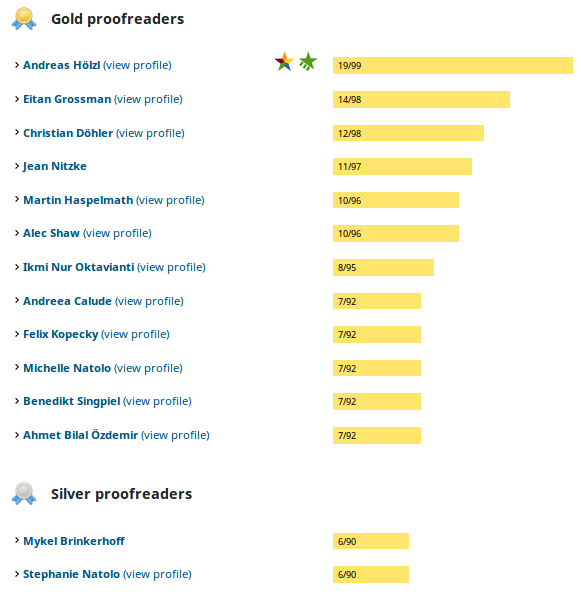
\includegraphics[height=1.5\textheight]{halloffame.png}
}

\frame{
\frametitle{Not a linguist?}
\begin{columns}
  \column{6cm}
  \begin{itemize}
    \item We wrote down our story, what worked, and what did not in the \textit{Cookbook for Open Access books}
    \item Freely available
    \item Complemented by the annotated business model
    \item   \url{https://zenodo.org/record/1286925}
    \item software, processes and business data are openly available as well
    \begin{itemize}
      \item https://userblogs.fu-berlin.de/langsci-press/2022/01/28/achievements-2021/
    \end{itemize}
  \end{itemize}
  \column{5cm}
  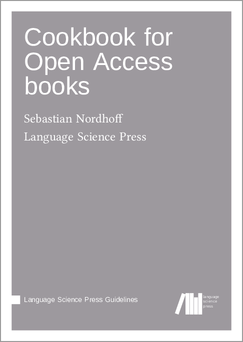
\includegraphics[height=.8\textheight]{cookbook.png} ~ \vfill ~
\end{columns}

}

\frame{
\frametitle{Thank you!}
  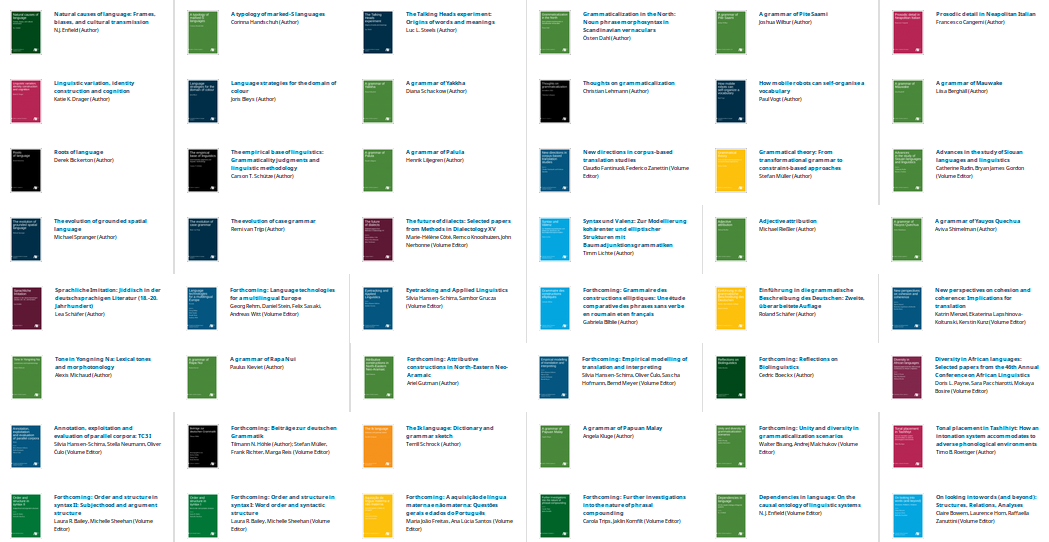
\includegraphics[height=\textheight]{catalog.png}
}

%\setcounter{framenumber}{\thelastpagemainpart}
\end{document}
